\chapter{Literature Review}
The field of Artificial Intelligence in healthcare is rapidly evolving, with significant advances in: (i) predictive diagnostic models \cite{optimizing_ai_sepsis_2024}, (ii) Multimodal data integration, and (iii) Explainable AI techniques. 

\section{AI in Healthcare}

\subsection{Surveys}
Here are some survey \& position papers. Rajpurkar et al. \cite{moor2023GMAI} advocate for \textit{generalist medical AI}, i.e. models which are trained on large, unlabelled, diverse datasets with self-supervision, can flexibly ingest different modalities (e.g. imaging, EHR, genomics) and produce expressive outputs (e.g. free-text explanations, spoken recommendations). They argue that such models will be capable of carrying out a diverse set of tasks using very little or no task-specific labelled data.

\todo[inline]{Add surveys on sepsis, etc.}


\subsection{Healthcare Applications}
\label{sec:healthcare_applications}

\subsubsection{Sepsis}
\label{sec:sepsis}
\textbf{Sepsis}  is a life-threatening organ dysfunction caused by a dysregulated host response to infection \cite{singer2016sepsis3}. It is a leading cause of morbidity and mortality in hospitals, with an estimated 11 million deaths annually \cite{rudd2020global}. Organ dysfunction can be identified as an acute change in total SOFA score
$\geq 2$ points consequent to the infection, Fig \ref{fig:sofa}. Prior sepsis definitions used two of 4 SIRS criteria, which are not specific to sepsis and can lead to overdiagnosis(patients who has SIRS but not sepsis).


% insert inline SOFA figure in images/sofa.png
\begin{figure}[h]
    \centering
    \begin{subfigure}{0.5\textwidth}
        \centering
        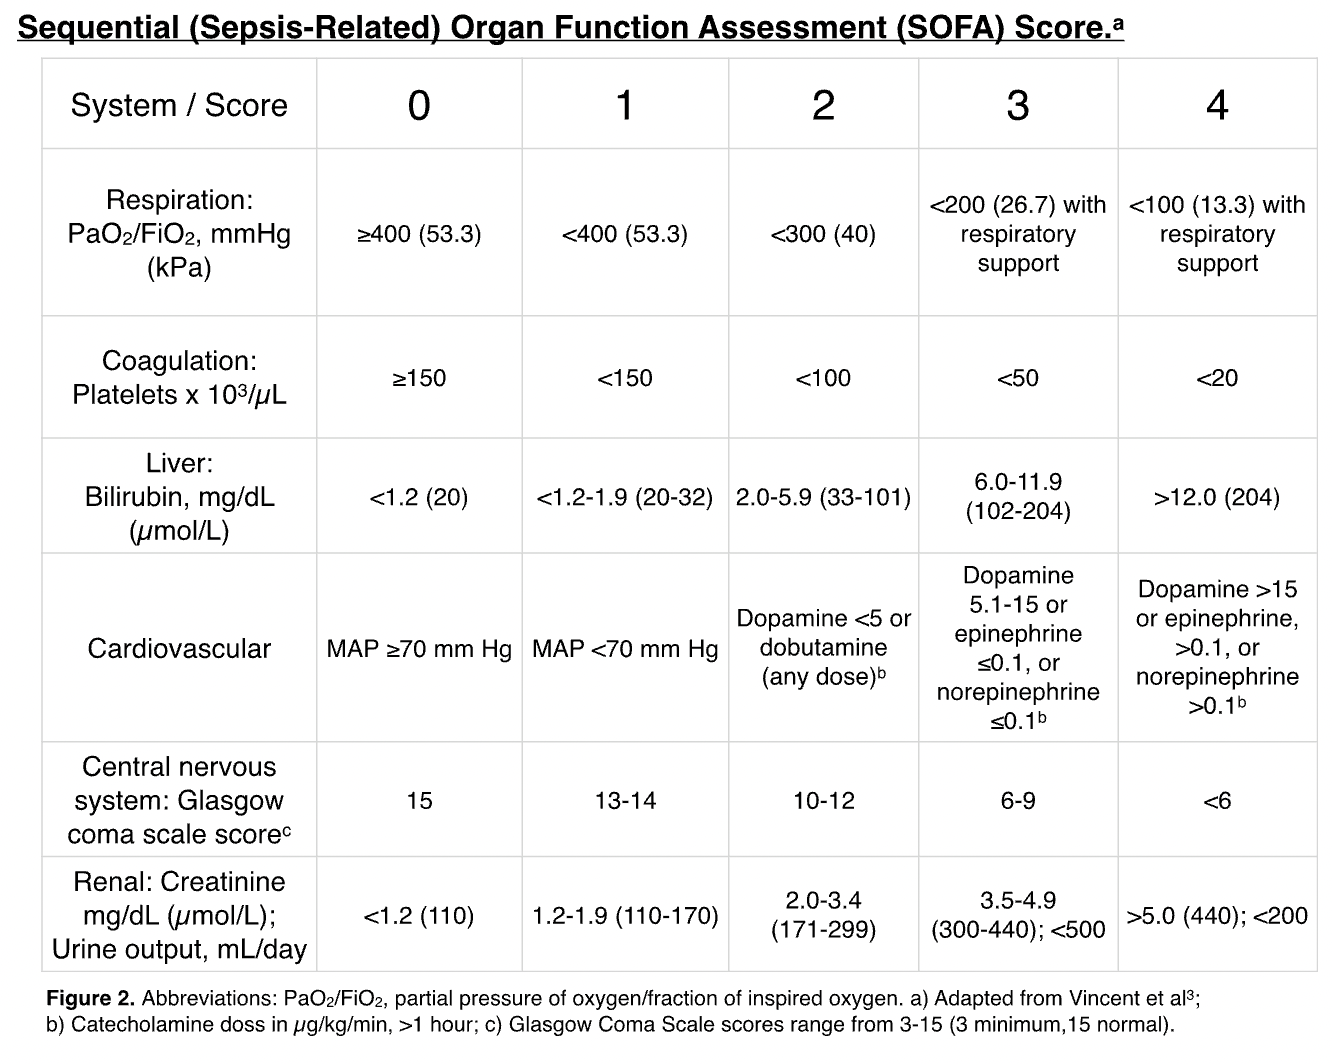
\includegraphics[width=\textwidth]{images/sofa.png}
        \caption{SOFA score criteria for organ dysfunction.}
        \label{fig:sofa}
    \end{subfigure}%
    \hfill
    \begin{subfigure}{0.5\textwidth}
        \centering
        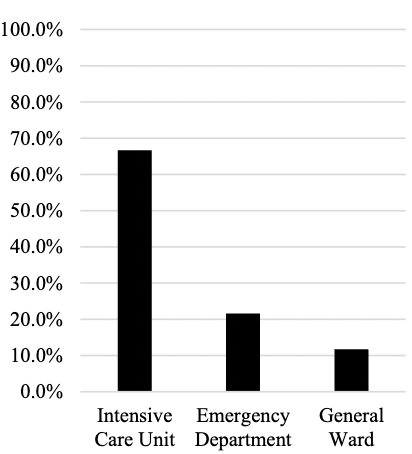
\includegraphics[width=\textwidth,height=0.25\textheight,keepaspectratio]{images/sepsis_datasources.png}
        \caption{Sepsis data sources.}
        \label{fig:sepsis_datasources}
    \end{subfigure}
    \caption{(a) SOFA score criteria for organ dysfunction and (b) Sepsis data sources.}
\end{figure}

The SOFA score is a clinical score used to track a patient's status during their stay in an ICU. It is used to determine the extent of a person's organ function or rate of failure. The SOFA score is based on the following six organ systems: respiratory, coagulation, liver, cardiovascular, renal, and neurological. Each system is assigned a score from 0 to 4, with higher scores indicating more severe dysfunction. The total SOFA score is the sum of the individual scores for each organ system.

\textbf{ML-Driven Sepsis Detection} \\ 
Surveys: Islam et al. \cite{islam2023survey} does a meta-study, showing that a majority of studies used ICU data (Fig \ref{fig:sepsis_datasources}), as well as the MIMIC-III dataset. Most of the studies were carried out using vital signs (73.1\%) and laboratory data (65.4\%).The median number of features was 22. The most common top features were heart rate, temperature, WBC count, systolic BP, age, dystolic BP and respiratory rate.


Moor et al. \cite{moor2021survey} show that . 


2025: \cite{Bignami2025AISepsis}
2025: FDA Device \cite{bhargava2024ImmunoScore}

HCI
2020: \cite{sandhu2022integrating}
2022: \cite{silvestri2022desired}


Papers
\textbf{2015-2017}: ?? 
\textbf{2017-2020}: TREWS \cite{adams2022trews} 
\textbf{2020-2022}: ??
\textbf{2023}: ??
\textbf{2024}: \cite{optimizing_ai_sepsis_2024}, \cite{zhang2024chi} shows that sepsis is uniquely high-stakes, uncertain, time-sensitive. Proposes an iterative loop where the model suggests labs to be drawn based on uncertainty.




\subsubsection{Cardiac Arrest}
\label{sec:cardiac_arrest}
\textbf{Cardiac Arrest} is a critical condition that requires immediate medical intervention. It occurs when the heart stops beating effectively, leading to a lack of blood flow to vital organs.  There are two types of cardiac arrest: out-of-hospital cardiac arrest (OHCA) and in-hospital cardiac arrest (IHCA). OHCA survival rate to discharge is 10-12\%, while IHCA survival rate is 20-25\% \cite{andersen2019cardiac}. 80\% of presenting rhythms are non-shockable, meaning that defibrillation is not an option, i.e. that early detection is the best fix. The incidence is 9-10 per 1000 admissions \cite{andersen2019cardiac}.

\textbf{Breast Cancer} affects 1 in 8 women. They use recurrence gene assays (Breast Cancer Index, JCO). 



\section{Explainable AI}
\todo[inline]{read the LIME, SHApe papers, and add a summary here.}

\section{Multimodal AI}
\todo[inline]{read the papers on multimodal AI, and add a summary here.}

RQ: how do we compress exomic analysis? 
Videos belong in low-dimensional space, so do sequences also?

Dimension-reduction with phenotypes! 

HeLM
HAIM 

\section{Time-Series Forecasting}

Given $\mathbf{X}$, a vector of time-series data, and a binary labelling function $f(\mathbf{X}, t)$ which labels the current state as 0/1, our task is to given $\mathbf{X}[i]$, predict $f(\mathbf{X}, j)$ for some $j > i$.

Approaches:
\begin{enumerate}
    \item Encode X[0...i] as text, ask an LLM
    \item Encode X[0...i] as text, fine-tune an LLM classification head
    \item Neurosymbolic: Somehow encode X[0...i], get distribution of $f(\hat{X}_{i+1}), f(\hat{X}_{i+2})...f(\hat{X}_{j})$, train a model with binary cross-entropy loss
    \item Neurosymbolic with Pretraining: Somehow encode X[0...i], First, pretrain a model M to do next-event prediction, i.e. given $\mathbf{X}[i]$, predict $\mathbf{X}_{i+1}, \mathbf{X}_{i+2}, ..., \mathbf{X}_{j}$, then fine-tune M using the neurosymbolic approach above.
\end{enumerate}




